\chapter{THIẾT KẾ CƠ KHÍ}
    \section{Tính toán và chọn động cơ}
        \subsection{Phân tích động lực học xe khi đi thẳng}
            \begin{figure}[H]
                \centering
                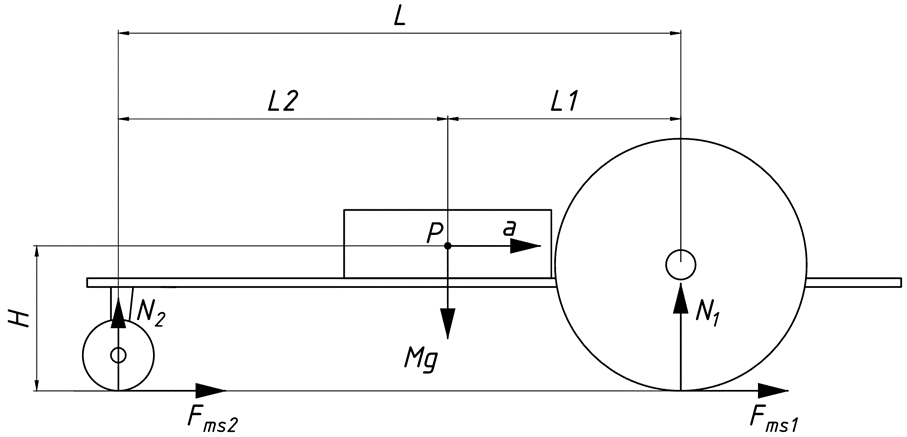
\includegraphics[width=1\textwidth]{pictures/chapter3/c3_p1_StraightAnalysis.png}
                \caption{Mô hình phân tích động lực học xe khi đi thẳng}
                \label{fig:3.1}
            \end{figure}
            \hspace*{0.6cm}Các thành phần lực:
            \begin{itemize}
                \item $N_1$ - Phản lực tại bánh dẫn động (N)
                \item $N_2$ - Phản lực tại bánh bị động trước (N)
                \item $N_3$ - Phản lực tại bánh bị động sau (N)
                \item $L = L_1 + L_2$ - Khoảng cách trục bánh trước và bánh sau (m)
                \item $H$ - Chiều cao từ trọng tâm xe đến mặt đất (m)
                \item $r$ - Bán kính bánh xe dẫn động (m)
                \item $M$ - Khối lượng của hệ (kg)
                \item $g = 9.8 \, m/s^2$ - Gia tốc trọng trường tại vị trí đang xét
                \item $a$ - Gia tốc của hệ ($m/s^2$)
            \end{itemize}
            \hspace*{0.6cm}Phương trình cân bằng lực:
            \begin{equation}
                \begin{cases}
                    \sum F_x = 0 \Rightarrow 2F_{ms1} + F_{ms2} = Ma \\
                    \sum F_y = 0 \Rightarrow 2N_1 + N_2 = Mg \\
                    \sum M_{z/c} = 0 \Rightarrow 2N_2L_1 - 2F_{ms2}H - 2F_{ms1}H - 2N_1L_1 - 2F_{ms1}H = 0
                \end{cases}
                \label{eq:3-1}
            \end{equation}
            \begin{equation}
                \Rightarrow
                \begin{cases}
                    2F_{ms1} + F_{ms2} = Ma  \\[0.2cm]
                    N_1 = \dfrac{MgL_2}{2L} - \dfrac{MaH}{2L} \\[0.2cm]
                    N_2 = \dfrac{MgL_1}{2L} + \dfrac{MaH}{2L}
                \end{cases}
                \label{eq:3-2}
            \end{equation}
        \subsection{Điều kiện để bánh xe luôn bám mặt đường}
            \hspace*{0.6cm}Để bánh xe luôn bám mặt đường thì phản lực tại điểm tiếp xúc giữa bánh xe và mặt đường luôn lớn hơn không khi đó:
            \begin{equation}
                \begin{cases}
                    N_1 = \dfrac{MgL_2}{2L} - \dfrac{MaH}{2L} \\[0.3cm]
                    N_2 = \dfrac{MgL_1}{2L} + \dfrac{MaH}{2L}
                \end{cases}
                \label{eq:3-3}
            \end{equation}
            \begin{equation}
                \Rightarrow
                L_{2}g > aH
                \label{eq:3-4}
            \end{equation}
        \subsection{Điều kiện để xe không bị lật khi vào cua}
            \begin{figure}[H]
                \centering
                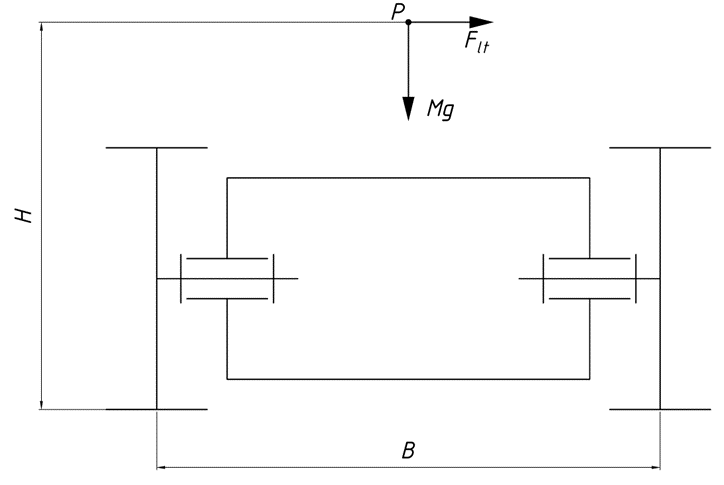
\includegraphics[width=0.6\textwidth]{pictures/chapter3/c3_p2_TurningAnalysis.png}
                \caption{Mô hình phân tích động lực học xe khi vào cua không lật}
                \label{fig:3.2}
            \end{figure}
            \hspace*{0.6cm}Để xe không lật thì momen do lực li tâm gây ra không lớn hơn moment do trọng lực gây ra:
            \begin{align}
                F_{lt}H &\leq P \times \dfrac{B}{2} \label{eq:3-5a} \\
                \Rightarrow \dfrac{B}{H} &\geq \dfrac{2F_{lt}}{Mg} \Rightarrow \dfrac{B}{H} \geq \dfrac{2Mv_{max}^2}{RMg} \label{eq:3-5b} \\ 
                \Rightarrow \dfrac{B}{H} &\geq \dfrac{2 \times 0.5^2}{0.5 \times 9.8} = 0.102 \label{eq:3-5c}
            \end{align}
            \hspace*{0.6cm}Trong đó: $v_{max} = 0.5$ m/s; $R = \rho_{min} = 0.5$ m; $g = 9.8$ m/s$^2$.
        \subsection{Điều kiện để xe không trượt khi vào cua}
            \begin{figure}[H]
                \centering
                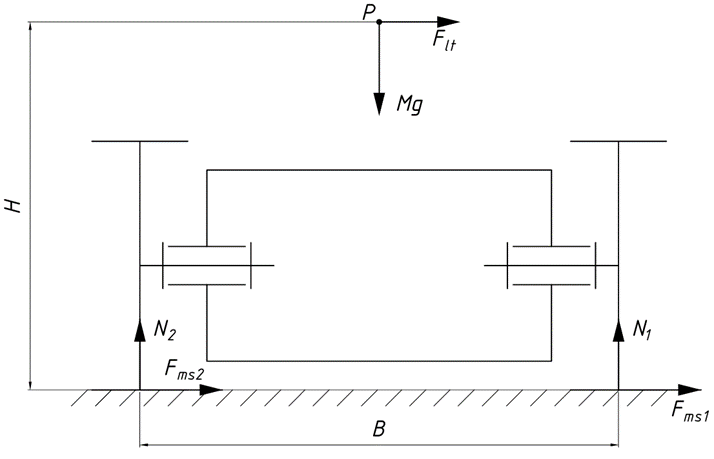
\includegraphics[width=0.6\textwidth]{pictures/chapter3/c3_p3_TurningAnalysis2.png}
                \caption{Mô hình phân tích động lực học xe khi vào cua không trượt}
                \label{fig:3.3}
            \end{figure}
            \hspace*{0.6cm}Để xe không trượt khi vào cua thì lực hướng tâm, trong trường hợp này là tổng lực ma sát tác dụng lên xe lớn hơn lực li tâm:
            \begin{align}
                \sum F_{ms} &\geq Ma_n \label{eq:3-12} \\
                \Rightarrow \mu Mg &\geq \dfrac{Mv_{max}^2}{r} \label{eq:3-13} \\
                \Rightarrow v_{max} &\leq \sqrt{\mu gR} \label{eq:3-14}
            \end{align}